\documentclass[12pt,a4paper]{report}

\usepackage{graphicx}
\graphicspath{{./}}
\usepackage{amsmath}
\usepackage{cite}
\usepackage{hyperref}
\usepackage{float}
\usepackage{geometry}

\geometry{margin=1in}

\begin{document}

% ============================================================
% TITLE PAGE
% ============================================================

\begin{titlepage}
\begin{center}

\vspace{0.5cm}

{\Huge\textbf{PROJECT TITLE}}

\vspace{1.5cm}

{\large A Lab Project Report submitted for the partial fulfillment of the degree of}

\vspace{0.5cm}

{\Large \textbf{Bachelor of Technology}}

\vspace{0.3cm}

{\large in}

\vspace{0.3cm}

{\Large \textbf{Computer Science and Engineering}}

\vspace{1.8cm}

{\large Submitted by}

\vspace{0.4cm}

{\large 
\textbf{Name — S22xxxx} \\
\textbf{Name — S22xxxx}
}

\vspace{2cm}


\includegraphics[width=4.5cm]{logo.png}

\vspace{0.5cm}

{\Large \textbf{Rajiv Gandhi University of Knowledge Technologies}}

\vspace{0.3cm}

{\large 
S.M. Puram, Etcherla Mandal \\
Srikakulam District, Andhra Pradesh \\
India – 532402
}

\vspace{0.5cm}

\end{center}
\end{titlepage}

% ============================================================
% CERTIFICATE
% ============================================================

\chapter*{\centering CERTIFICATE}

\begin{center}

\includegraphics[width=0.25\textwidth]{logo.png}
\end{center}

\vspace{1cm}

This is to certify that the Lab Project entitled \textbf{``Your Project Title''}
submitted by \textbf{Name1 (ID)} and \textbf{Name2 (ID)} in partial fulfillment 
of the requirements for the Data Science with Python Lab Project.

\vspace{6cm}

\begin{center}
\begin{tabular}{p{5cm} p{5cm} p{5cm}}

 & & \centering Faculty Signature \\

\end{tabular}
\end{center}

% ============================================================
% ABSTRACT
% ============================================================

\chapter*{\centering ABSTRACT}

Briefly describing the problem your project solves.

\tableofcontents
\listoffigures

\newpage

% ============================================================
% CHAPTER 1: Introduction
% ============================================================

\chapter{Introduction}

This chapter introduces the project background and objectives.

\section{Background}
Explain the background of the project.

\section{Problem Statement}
Describe the problem your project solves.

\section{Objectives}

\begin{itemize}
\item Objective 1
\item Objective 2
\item Objective 3
\end{itemize}

\section{Organisation of Report}

Explain report organisation.

% ============================================================
% CHAPTER 2: Data Preprocessing
% ============================================================

\chapter{Data Preprocessing}

Briefly describe Data Preprocessing.

\begin{figure}[H]
\centering
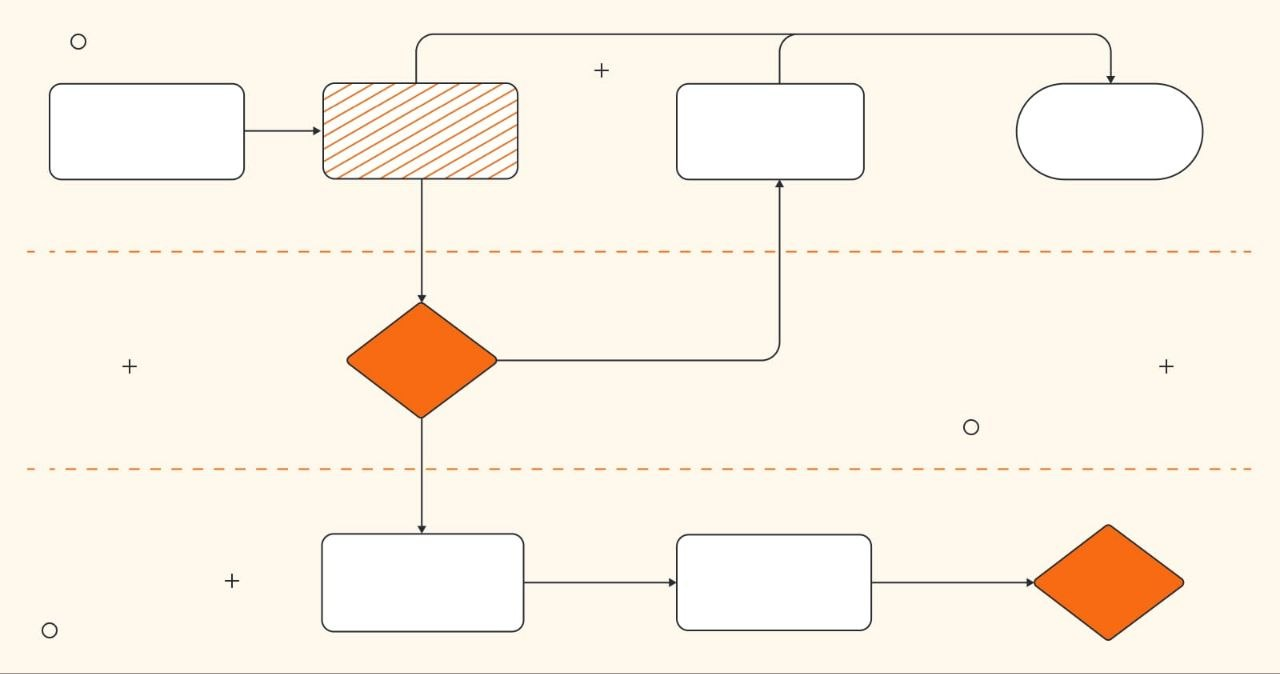
\includegraphics[width=0.75\textwidth]{image.png}
\caption{Example Figure}
\end{figure}

% ============================================================
% CHAPTER 3: Data Visualization
% ============================================================

\chapter{Data Visualization}

Briefly describe Data Visualization.

\begin{figure}[H]
\centering
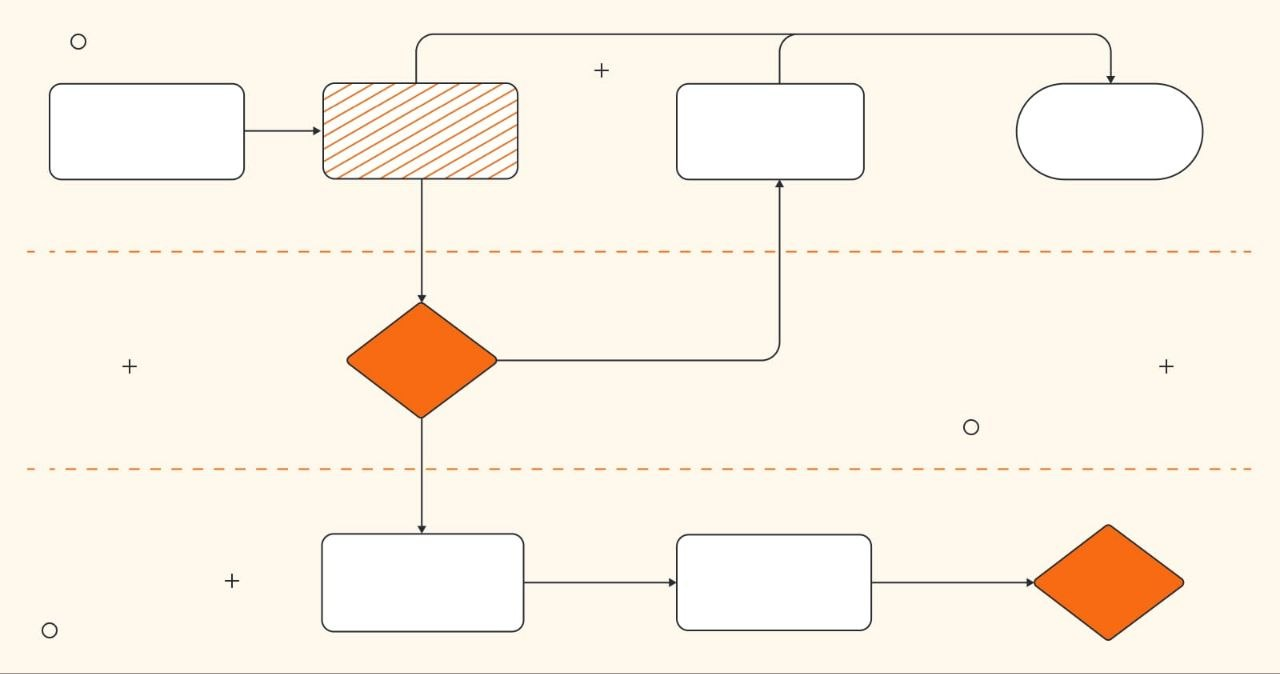
\includegraphics[width=0.75\textwidth]{image.png}
\caption{Example Figure}
\end{figure}

% ============================================================
% CHAPTER 4: Model Fitting
% ============================================================

\chapter{Model Fitting}

Briefly describe Model Fitting.

\begin{figure}[H]
\centering
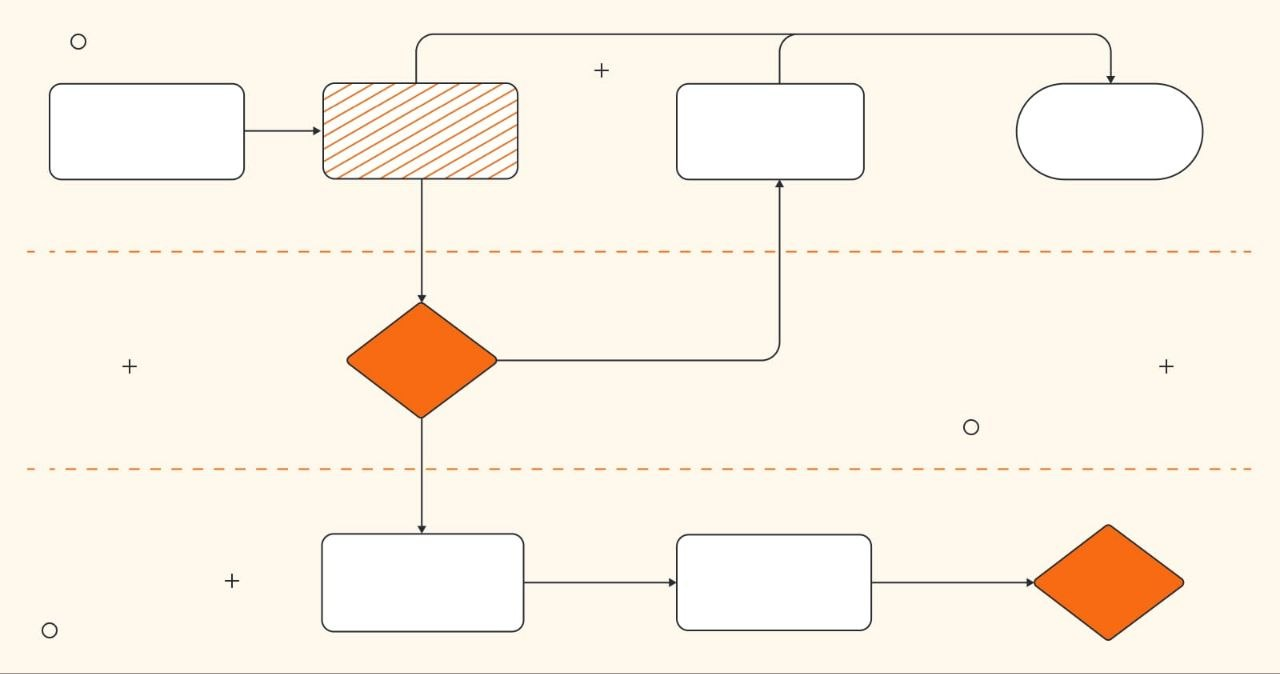
\includegraphics[width=0.75\textwidth]{image.png}
\caption{Example Figure}
\end{figure}

% ============================================================
% CHAPTER 5: References
% ============================================================

\chapter{References}

Attach the links and citations referred to build this project.

\begin{itemize}
\item Reference 1
\item Reference 2
\item Reference 3
\end{itemize}

\end{document}